To assess our neural network extrapolation method, we want to compare it to classical, state-of-the-art model-space extrapolations. Classical extrapolations are usually done using exponential fits. Even though the convergence of ground state energy sequences does not resemble an exponential convergence, it provides a good estimate on the ground-state energy. To ensure comparability, the classical extrapolation method is restricted to the same $N_\mathrm{max}$ values as in the neural network extrapolation, such that the input sequences are formatted exactly as described earlier, using all subsets of 3 out of all available oscillator frequencies.


In a classical extrapolation, an exponential function
\begin{equation}
  \label{eqn:cl_extr}
  f(x) = a \exp(-bx) + c
\end{equation}
is fitted on a sequence of three $N_\mathrm{max}$ values with a specific oscillator frequency. The resulting limit value $c$ can then be extracted as as the extrapolated value of the ground-state energy. Out of all available frequencies, we choose the frequency which has the lowest energy value at the highest $N_\mathrm{max}$. This is motivated by the fact that these sequences are usually more converged, which ensures more precision in the function fit.

\begin{figure}[H]
  \centering
  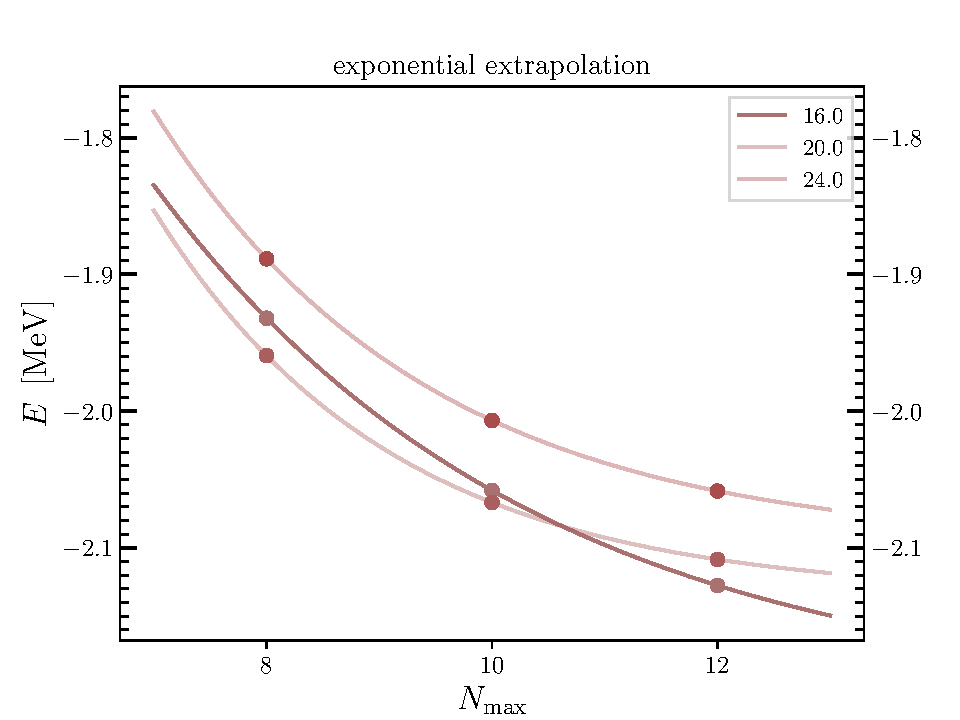
\includegraphics[width=.5\textwidth]{media/example_cl_extr.pdf}
  \caption{For the three different frequencies of $\hbar\Omega = 16, 20, 24$, a function fit of \autoref{eqn:cl_extr} is shown. For the extrapolated ground-state energy, the function fit of the squence with the lowest value for the highest $N_\mathrm{max}$ is chosen. In this example, it is the frequency $\hbar\Omega=16$}
  \label{fig:example_cl_extr}
\end{figure}
For example, if we wanted to extrapolate the sample in \autoref{fig:example_evaluation} with frequencies $\hbar\Omega = 16, 20, 24$ for the case of maximum $N_\mathrm{max}$ of 12, we choose the values  $N_\mathrm{max} = 8, 10, 12$ of the $\hbar\Omega = 16$ sequence for extrapolation, since the absolute value of its sequence is the lowest among the three frequencies at $N_\mathrm{max} = 12$. The resulting function fit is shown in \autoref{fig:example_cl_extr}
